\chapter{Monitoring and Governance}
\label{chap:monitoring}

This chapter describes how the pipeline observes operational risk after inference and how that
observation is converted into a governed decision. The architecture in Chapter~\ref{chap:architecture}
separated the operational assessment path (Stages~1--7) from the governed mutation path
(Stages~8--10). Monitoring (Stage~6) and trigger evaluation (Stage~7) are the part of the assessment
path that turns raw predictions into a risk assessment, and they are the mechanism that keeps model
mutation explicitly gated rather than automatic. Monitoring is therefore part of the runtime control logic, not an optional layer added after inference.

\section{Why Monitoring Is Needed Under Label-Scarce Operation}
\label{sec:why_monitoring}

When a model is evaluated on a labeled test set, its behavior can be summarized with accuracy,
macro-F1, and a confusion matrix. In deployment-style wearable monitoring this assumption breaks
down, because ground-truth labels are usually unavailable when a new session arrives. The system can
still generate predictions, but it cannot immediately verify whether those predictions are correct.
The pipeline must therefore rely on \emph{proxy} signals that indicate operational risk even when
direct performance metrics cannot be computed~\cite{bodor2023mlopsmonitoring}.

The thesis treats these proxy signals as a control layer. Stage~6 observes the run and rates its
behavior; Stage~7 converts that behavior into a single governance action. Neither stage mutates the
active model. This preserves the central architectural rule that observation and mutation are
separated: the system can detect that a session may be unreliable without assuming that automatic
retraining is the correct response.

\section{Post-Inference Monitoring}
\label{sec:three_layer_monitoring}

Stage~6 is warning-oriented and non-mutating. It evaluates three complementary signal layers plus a
collapse-risk check. The first layer is confidence and uncertainty, which captures how decisive the
model is per window. The second layer is temporal behavior, which captures how often the predicted
class switches between neighboring windows. The third layer is distribution drift, which compares
incoming sensor windows against a reference baseline. The monitor also tracks
dominant-class concentration, because a model that assigns most windows to a single class is a
characteristic failure mode in label-scarce operation. Each signal is rated relative to a conservative
operating threshold, summarized in Table~\ref{tab:monitoring_signals}. How these threshold values were chosen, together with the calibration evidence behind them, is set out in Section~\ref{sec:threshold_scope}.

\renewcommand{\arraystretch}{1.2}
\begin{table}[htbp]
\centering
\footnotesize
\caption[Stage~6 monitoring signals and their conservative operating thresholds]{Stage~6 monitoring signals and their conservative operating thresholds. None of these
signals requires ground-truth labels; each indicates operational risk rather than verified error.}
\label{tab:monitoring_signals}
\begin{tabularx}{\textwidth}{p{3.2cm} X p{3.0cm}}
\toprule
\textbf{Signal} & \textbf{What it measures} & \textbf{Warning threshold} \\
\midrule
Mean confidence & Per-window decisiveness of the softmax output. & below \(0.70\) \\
Uncertain-window rate & Share of windows whose confidence falls below the uncertainty level. & above \(20\%\) \\
Transition rate & How often the predicted class changes between adjacent windows. & above \(35\%\) \\
Drift (z-score) & Distance of incoming windows from the training-distribution baseline. & above \(1.8\) \\
Dominant-class share & Fraction of windows assigned to the single most frequent class. & \(85\%\) warn / \(95\%\) critical \\
\bottomrule
\end{tabularx}
\renewcommand{\arraystretch}{1.0}
\end{table}

The choice of signals reflects distinct failure modes that arise in label-scarce wearable monitoring, each invisible to at least one of the other signals.

Confidence is taken directly from the model's softmax output: for each window the predicted-class probability is its confidence, and a run is summarized by the mean confidence and by the share of windows whose confidence falls below an uncertainty level. This signal is the model's own native output, requires no labels, and is essentially free to compute. It is deliberately not trusted in isolation, because softmax confidence is frequently miscalibrated (Section~\ref{sec:calibration_gap}); its role is to flag low-decisiveness runs and to contribute one vote to the trigger policy, not to certify correctness.

The transition rate measures how often the predicted class changes between adjacent windows. The target behaviors persist over several seconds while the windowing emits a new prediction every two seconds, so genuine activity should produce mostly stable neighboring predictions and frequent switching indicates an unstable output sequence. The transition rate is independent of confidence: a model can be confident on each individual window yet flip between classes from one window to the next, a pattern that a confidence threshold alone would miss.

Drift compares the incoming sensor windows against the training-distribution baseline using a per-channel z-score statistic. A z-score is used at runtime rather than a heavier two-sample test because it is lightweight, fast, and directly comparable across the six channels, which suits the offline-first, per-session setting; a more sensitive kernel-based statistic (MMD) is retained only as an offline audit branch (Section~\ref{sec:mmd_audit}), since the runtime monitor needs to surface a shift for review rather than characterize it precisely. Drift can detect a change in the input itself (a different device, placement, or unit convention) before that change appears as a collapse in the output~\cite{gama2014survey,webb2016characterizing}. Two drift baselines are active in the system, one per serving path. The API path compares scaled windows against the normalized baseline inside the runtime-contract folder; the batch pipeline's Stage~6 uses a raw-physical-units baseline, matching the physical space in which its windows are audited. In both paths, if the baseline is missing or its feature space does not match the production windows, Stage~6 routes the condition to review rather than fabricating a drift result from incompatible spaces, consistent with the runtime-contract discipline of Chapter~\ref{chap:data_model}.

The dominant-class share is the fraction of windows assigned to the single most frequent class. It is tracked because dominant-class collapse is invisible to confidence: a collapsed model can assign almost every window to one class with high confidence. Measuring output concentration directly therefore catches a failure that the other signals would not, and it is the signal most directly tied to the collapse guard in Stage~7 (Section~\ref{sec:trigger_policy}).

The formal definitions used throughout the chapter follow from this signal set. Let a session produce $N$ windows. For window $i$ the model outputs a softmax vector $\mathbf{p}_i=(p_{i,1},\dots,p_{i,K})$ over the $K=11$ classes; the predicted class is $\hat{y}_i=\arg\max_k p_{i,k}$ and the per-window confidence is $c_i=\max_k p_{i,k}$. The mean confidence and the uncertain-window rate are
\[
\bar{c}=\frac{1}{N}\sum_{i=1}^{N}c_i,
\qquad
U=\frac{1}{N}\sum_{i=1}^{N}\mathbf{1}\!\left[c_i<\tau_u\right],
\]
where $\tau_u$ is the uncertainty level; a run is flagged when $\bar{c}<0.70$ or $U>0.20$. A complementary uncertainty measure is the predictive entropy of each window,
\[
H_i=-\sum_{k=1}^{K}p_{i,k}\log p_{i,k},
\]
which is computed by the optional calibration stage rather than by the defended Stage~6 signal set; it is defined here for completeness because the calibration analysis of Chapter~\ref{chap:experiments} draws on it. The transition rate, which captures temporal stability, is
\[
T=\frac{1}{N-1}\sum_{i=2}^{N}\mathbf{1}\!\left[\hat{y}_i\neq\hat{y}_{i-1}\right],
\]
flagged when $T>0.35$. This rate is computed on the raw per-window prediction stream so that it remains a faithful instability signal. In the serving path, the activity sequence returned to the operator is additionally passed through a majority-vote temporal smoothing over neighboring windows, the decision stage of the activity-recognition chain~\cite{bulling2014tutorial,lester2006practical}, which suppresses isolated single-window flips without altering the monitored value of~$T$. With class counts $n_k=\sum_{i=1}^{N}\mathbf{1}[\hat{y}_i=k]$, the dominant-class share is
\[
D=\frac{1}{N}\max_{k}n_k,
\]
with a warning at $D\ge0.85$ and a critical level at $D\ge0.95$. Distribution drift standardizes each channel statistic against the training baseline: if channel $j$ has baseline mean $\mu_j$ and standard deviation $\sigma_j$ and the incoming session has channel mean $\hat{\mu}_j$, the drift score is
\[
z=\max_{j}\frac{\lvert \hat{\mu}_j-\mu_j\rvert}{\sigma_j},
\]
flagged when $z>1.8$. Because $z$ compares per-channel session \emph{means} only, it is intentionally blind to variance and higher-moment shift: a session could match all six channel means while differing in amplitude spread or spectral content and still produce $z\approx0$. This blind spot is accepted at runtime for the sake of a cheap, interpretable statistic; the offline MMD audit branch exists precisely to cover it. The optional audit branch instead measures the Maximum Mean Discrepancy between a reference sample $X=\{x_i\}_{i=1}^{n}$ and an incoming sample $Y=\{y_j\}_{j=1}^{m}$ under a kernel $k(\cdot,\cdot)$,
\[
\mathrm{MMD}^2(X,Y)=\frac{1}{n^2}\sum_{i,i'}k(x_i,x_{i'})+\frac{1}{m^2}\sum_{j,j'}k(y_j,y_{j'})-\frac{2}{nm}\sum_{i,j}k(x_i,y_j),
\]
which is more sensitive but computationally heavier, and is therefore reserved for offline auditing rather than per-session runtime use~\cite{gretton2012kernel}.

\subsection{Confidence Limits and the Calibration Gap}
\label{sec:calibration_gap}

Confidence is a useful but limited signal. A high softmax probability suggests that the model is
decisive, but it does not guarantee that the prediction is correct, because modern neural networks
are frequently poorly calibrated~\cite{guo2017calibration,blasiok2024calibration}. This limitation is
not hypothetical in this thesis. On the external User~7 probe, the model produced a mean softmax
confidence of approximately \(0.86\) while its labeled accuracy (reported in
Chapter~\ref{chap:experiments}) was far lower. The dominant failure mode is therefore
\emph{high-confidence misprediction}, not low-confidence uncertainty.

This has a direct design consequence: a single threshold on confidence cannot catch a
confident-but-wrong session. If confidence were the only monitored signal, such a run would pass
silently. For this reason the monitor combines confidence with temporal, drift, and
dominant-class signals, and the trigger policy requires agreement across signals rather than trusting
any one of them. Bayesian uncertainty approximations such as Monte~Carlo dropout~\cite{gal2016dropout}
provide a complementary view of predictive instability and are treated as an optional extension rather
than as a defended runtime property.

\section{Trigger Policy and Governance}
\label{sec:trigger_policy}

Stage~7 converts the Stage~6 signals, together with collapse evidence, into a single governance
action. The collapse guard is evaluated first: if a collapse condition holds, such as a
dominant-class share at or above \(95\%\), or a high-confidence single-class pattern with no
temporal variation, the action is review with \texttt{should\_retrain=false}, regardless of the other
signals. If no collapse is detected, the confidence, temporal, and drift signals are scored and
aggregated by voting under an explicit no-auto-retrain policy. Any critical signal escalates to
review; two or more warnings route the session to a review and label queue; a single warning is
logged for monitoring; otherwise the run is healthy. Consecutive-warning escalation promotes repeated
warnings to review without ever setting an automatic trigger, and a cooldown gate is applied last to
prevent rapid retraining loops. Table~\ref{tab:trigger_decisions} summarizes this mapping, and
Figure~\ref{fig:monitoring_governance_flow} shows the overall flow.

The rationale for this design is that no single signal is trustworthy on its own, so the policy is built around agreement rather than any one threshold. Voting lets a confident-but-wrong run still be caught when temporal instability or drift disagrees with the confidence signal, while requiring more than one warning before escalation keeps the false-alarm rate low. The thresholds are deliberately tiered, with monitoring warnings firing earlier and the trigger applying stricter limits, so that risk becomes visible well before any mutation is even considered. Above all the policy is asymmetric: it is easy to raise a review, while by construction no code path converts signal severity into automatic mutation without the label and quality-assurance gate, because retraining from unlabeled, shifted, or collapsed predictions can reinforce the model's own errors. The benefit of the trigger layer is therefore measured not by how often it retrains, but by how reliably it routes genuinely risky sessions to human review while leaving the model unchanged.

Formally, after the collapse guard, let $w$ and $c$ be the numbers of warning- and critical-level signals among confidence, temporal, and drift. The governance action is
\[
a=\begin{cases}
\texttt{review} & \text{collapse guard holds, or } c\ge 1,\\
\texttt{queue\_retrain} & c=0 \text{ and } w\ge 2,\\
\texttt{monitor} & c=0 \text{ and } w=1,\\
\texttt{none} & w=c=0,
\end{cases}
\]
with \texttt{should\_retrain}$=$\texttt{false} enforced for unlabeled production data in every case, and a final cooldown gate that rewrites a would-be retraining candidate into a queued review.

\renewcommand{\arraystretch}{1.2}
\begin{table}[htbp]
\centering
\footnotesize
\caption[Stage~7 trigger decisions under the no-auto-retrain policy]{Stage~7 trigger decisions under the no-auto-retrain policy. Severity never authorizes
mutation on its own; unlabeled production data cannot trigger automatic retraining.}
\label{tab:trigger_decisions}
\begin{tabularx}{\textwidth}{p{4.2cm} X}
\toprule
\textbf{Signal pattern} & \textbf{Governance action} \\
\midrule
Collapse condition holds & \texttt{review}; \texttt{should\_retrain=false} (checked first, overrides voting). \\
Any critical signal & \texttt{review} required; no trigger. \\
Two or more warnings & \texttt{queue\_retrain} (review/label queue; \texttt{label\_required=true}); no immediate mutation. \\
One warning & \texttt{monitor}; no trigger. \\
No warnings & Healthy; no action. \\
Cooldown active (final gate) & Decision rewritten to \texttt{queue\_retrain}; \texttt{should\_trigger=false}. \\
\bottomrule
\end{tabularx}
\renewcommand{\arraystretch}{1.0}
\end{table}

Stage~6 and Stage~7 thresholds are intentionally tiered: the monitoring warning thresholds are
earlier and looser, while the trigger thresholds are stricter governance limits (for example, the
trigger treats confidence below \(0.65\) as a warning and below \(0.50\) as critical, drift z-scores
above \(2.0\) and \(3.0\) as warning and critical, and applies a \(24\)-hour cooldown). The two
stages share signal names but serve different purposes, so their thresholds differ deliberately:
Stage~6 is tuned for \emph{sensitivity}, because its warnings only create visibility in session
reports and a false warning costs little, while Stage~7 is tuned for \emph{specificity}, because its
output feeds the governance decision and a false trigger consumes review capacity. The trigger
levels follow a sigma rationale on the training distribution (a drift $z$ of \(2.0\) corresponds
roughly to the 95th percentile and \(3.0\) to the 99.7th~\cite{page1954cusum}), and the voting and
cooldown defaults are justified empirically by the calibration study reported in
Section~\ref{sec:ch7_triggerpolicy}.
Figure~\ref{fig:ch6_tiered} visualizes this tiering for the three voting signals.

\begin{figure}[htbp]
\centering
\makebox[\textwidth][c]{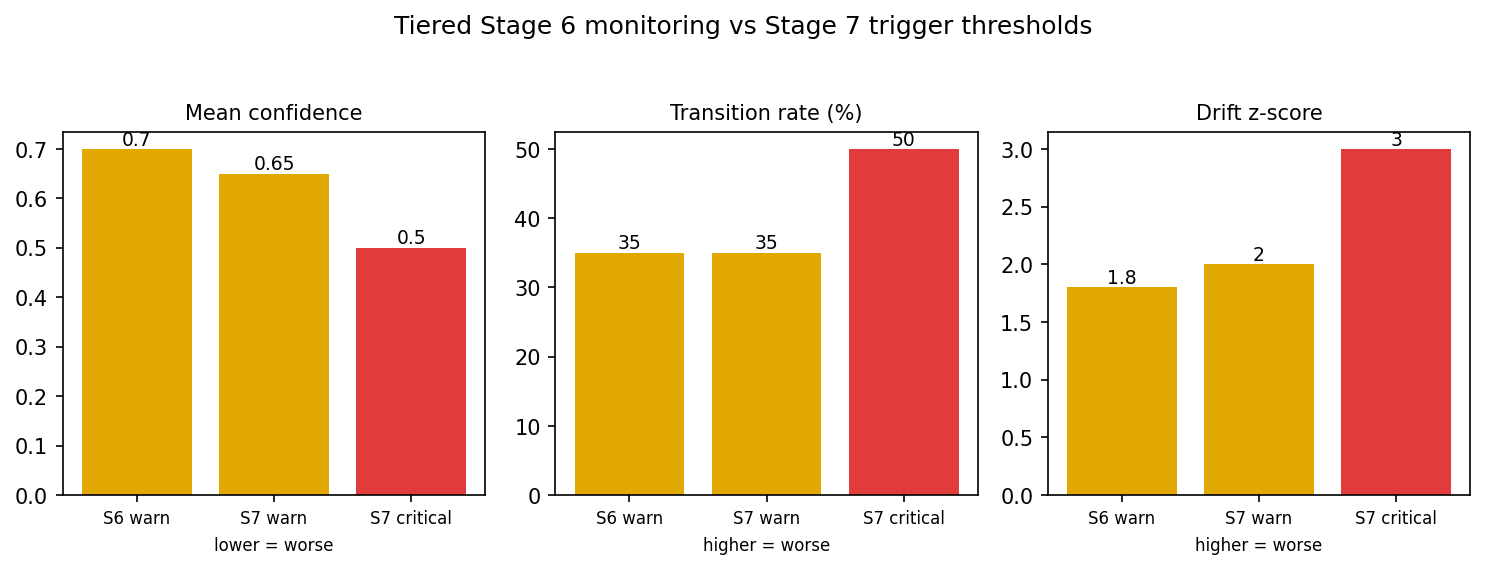
\includegraphics[width=1.12\textwidth]{figures/Figure_6_2_tiered_thresholds.png}}
\caption[Tiered thresholds for the three trigger-voting signals]{Tiered thresholds for the three
trigger-voting signals. For each signal, Stage~6 (monitoring) warns earlier and looser than
Stage~7, which adds a stricter warning and a critical limit before any governance vote is cast.}
\label{fig:ch6_tiered}
\end{figure}
\FloatBarrier

The tiering is deliberate and follows the same logic for all three signals. For confidence,
Stage~6 warns when the session mean drops below \(0.70\), while Stage~7 registers a governance
warning only below \(0.65\) and escalates to critical below \(0.50\). For the temporal transition
rate, Stage~6 flags instability at \(35\%\), while Stage~7 adds a critical boundary at \(50\%\)
before casting a vote. For distribution drift, Stage~6 raises a visibility flag at $z>1.8$, below
the Stage~7 governance warning at $z>2.0$ and the critical level at $z>3.0$. The gap between the
Stage~6 and Stage~7 warning boundaries is the sensitivity buffer: a run sitting between the two
levels is visible in session reports without consuming governance review capacity.

Stage~7 converts the per-layer signals from Stage~6 into a single governance action through a
four-step evaluation sequence. A collapse guard is applied first to catch cases where the
model output has concentrated on one class regardless of the individual signal levels; the
remaining signals are then aggregated by a voting rule across L1--L3; persistent low-level
risk is escalated when the same single-warning pattern repeats across consecutive runs; and a
cooldown gate prevents duplicate triggers within 24 hours of a recent retrain.
The full path, from the Stage~4 softmax output through Stage~6 monitoring to the final
governance action, is illustrated in Figure~\ref{fig:monitoring_governance_flow}.

\begin{figure}[htbp]
\centering
\begin{tikzpicture}[
  node distance=5mm,
  box/.style={rectangle, rounded corners=4pt, draw, align=left,
              text width=10.2cm, inner sep=8pt, font=\footnotesize},
  s4/.style={box, fill=gray!22},
  s6/.style={box, fill=blue!18},
  s7/.style={box, fill=orange!30},
  gov/.style={box, fill=green!22},
  arr/.style={-{Latex[length=2.5mm]}, thick}
]

\node[s4] (s4) {%
  \textbf{Stage~4: Predictions}\\[3pt]
  Softmax vector $\mathbf{p}_i$ over $K{=}11$ classes;\enskip
  confidence $c_i = \max_k p_{i,k}$;\enskip
  predicted class $\hat{y}_i = \arg\max_k p_{i,k}$
};

\node[s6, below=of s4] (s6) {%
  \textbf{Stage~6: Monitoring}\enskip\textit{(warning-only, non-mutating)}\\[3pt]
  L1:\enspace session mean confidence and uncertain-window rate\\[1pt]
  L2:\enspace temporal transition rate (raw and smoothed)\\[1pt]
  L3:\enspace per-channel distribution drift (z-score vs baseline)\\[1pt]
  \phantom{L3:}\enspace dominant-class concentration (collapse proxy signal)
};

\node[s7, below=of s6] (s7) {%
  \textbf{Stage~7: Trigger Policy}\enskip\textit{(\texttt{auto\_retrain=false} on all paths)}\\[3pt]
  1.\enspace Collapse guard (checked first; overrides voting if any condition holds)\\[1pt]
  2.\enspace Signal voting: $w$ warnings and $c$ critical signals among L1--L3\\[1pt]
  3.\enspace Consecutive-warning escalation: repeated $w{=}1$ promoted to review\\[1pt]
  4.\enspace Cooldown gate (24\,h): suppresses duplicate triggers
};

\node[gov, below=of s7] (gov) {%
  \textbf{Governance Action}\enskip\textit{(\texttt{should\_retrain=false} enforced)}\\[3pt]
  \texttt{none}:\enspace all signals healthy\\[1pt]
  \texttt{monitor}:\enspace single warning ($w{=}1$)\\[1pt]
  \texttt{review}:\enspace collapse guard triggered, or any critical signal ($c{\ge}1$)\\[1pt]
  \texttt{queue\_retrain}:\enspace two or more warnings ($w{\ge}2$); label and QA gate required
};

\draw[arr] (s4) -- (s6);
\draw[arr] (s6) -- (s7);
\draw[arr] (s7) -- (gov);

\end{tikzpicture}
\caption[Post-inference monitoring and governance flow]{Post-inference monitoring and governance
flow. Stage~6 evaluates three signal layers and a dominant-class collapse proxy; Stage~7
converts the signals into a governance action through a collapse guard, signal voting,
consecutive-warning escalation, and a cooldown gate. Signal severity never authorizes automatic
mutation: unlabeled production data routes to review or a label queue only.}
\label{fig:monitoring_governance_flow}
\end{figure}
\FloatBarrier

Both execution paths write their outputs to MLflow under two nested experiments. The inference
child run records the mean prediction confidence, the total window count, and individual
prediction counts for each of the eleven activity classes, together with the model content hash
and the runtime mode. The pipeline parent run aggregates the signals that drive the trigger
decision: mean confidence, dominant-activity share, distribution drift score, temporal transition
rate, an overall health flag, the alert severity level, and the retraining decision flag.
Separating the two runs lets a reviewer inspect the raw per-class prediction counts from the
inference stage independently of the aggregated signals the trigger policy actually consumes.
Neither run logs model weights or training data; the only artifact written is the monitoring
report, keeping the tracking store lightweight and audit-focused rather than a data archive.
Annotated screenshots of both experiments, including the run list, metric tab, and logged
artifacts for each path, are provided in Appendix~\ref{app:walkthrough}.

\subsection{Collapse Guard and Cooldown Semantics}
\label{sec:collapse_cooldown}

The collapse guard and the cooldown gate are the two mechanisms that keep the policy conservative in practice. The collapse guard is evaluated before the signal voting and returns a review action whenever any of the following conditions holds: an upstream dominance warning is raised; the dominant-class share reaches at least \(95\%\); the dominant-class share reaches at least \(90\%\) together with a zero transition rate and high confidence; Stage~4 reports a critical-collapse level; or Stage~6 flags a low-motion collapse risk. In every one of these cases the decision is \texttt{review} with \texttt{should\_retrain=false}, never automatic retraining, because a confidently collapsed single-class output is exactly the pattern that the confidence signal alone can miss.

The cooldown gate is applied last and has precedence over same-cycle escalation. If a decision would otherwise generate a retraining candidate while a recent retrain is still within the cooldown window (\(24\) hours by default), the final decision is rewritten to a queued review with \texttt{cooldown\_active=true}. The gate exists because consecutive sessions from the same wearer and device tend to share the conditions that raised the first alarm: without a cooldown, every such session would raise a near-duplicate retraining request, flooding the human review queue faster than it can be processed while adding no new information. This is particularly relevant in the offline-first setting, where multiple sessions from the same wearer may be processed in close succession and can reflect the same unresolved condition, such as a sensor placement issue, a domain shift, or an unusual movement style, rather than independent failures. Suppressing the duplicate trigger is safe because the underlying review remains open until a human closes it. The calibration study of Section~\ref{sec:ch7_triggerpolicy} quantifies this effect: the 24-hour cooldown reduces trigger volume from 164 to 14 on the recorded history while keeping precision at 1.0. Enforcing the cooldown after the escalation logic ensures that it cannot be overridden later in the same evaluation cycle. The collapse guard and the cooldown gate jointly guarantee that neither a single collapsed batch nor a rapid sequence of back-to-back runs can drive the system into automatic mutation.

\subsection{Severity Is Not Retraining: The Governance Boundary}
\label{sec:governance_boundary}

A central claim of this thesis is that monitoring severity and model mutation are two separate
decisions. A critical monitoring signal indicates observed risk above the warning threshold; it does
not prove that the model is wrong, and it does not prove that retraining would improve the system. On
both defended evidence runs the governance outcome is \texttt{action=review} with
\texttt{should\_retrain=false}: the run is flagged for human review, but no mutation stage is entered.
This is a deliberate governance policy, not a missing feature.

The justification is strongest precisely in the label-scarce setting. If the system retrained directly
from its own predictions on unlabeled, shifted, or collapsed data, it could reinforce its own errors
through confirmation bias~\cite{lee2013pseudolabel,arazo2020pseudolabel}. The policy therefore
requires that unlabeled production data never triggers automatic retraining regardless of signal
severity; a label and quality-assurance gate is required before any retraining candidate is even
generated.

\subsection{Retraining and Baseline Governance}
\label{sec:retraining_governance}

The mutation path (Stages~8--10) is reached only after the governance conditions are satisfied. Stage~8
generates a retraining candidate, Stage~9 registers it with provenance, and Stage~10 promotes it to the
active runtime contract. Each step is conditional on review, labels, and validation evidence, and the
cooldown gate prevents back-to-back retraining loops by rewriting a would-be trigger into a queued
review when a recent retrain is still within the cooldown window. If a candidate fails validation or
later proves unsuitable, the previous runtime package remains available as a rollback reference. This
keeps mutation reviewable and reversible rather than automatic, consistent with the same-folder
runtime-contract rule of Chapter~\ref{chap:architecture}.

\section{Evaluation Metrics: Labeled and Unlabeled Conditions}
\label{sec:evaluation_metrics}

The metrics available to the system depend on whether labels are present. Under labeled evaluation, the
pipeline can compute accuracy, macro-F1, and a confusion matrix, which are reported in
Chapter~\ref{chap:experiments}. Under unlabeled deployment-style operation, only proxy metrics are
available: mean confidence, uncertain-window rate, transition rate, dominant-class share, and drift
distance. These proxy metrics indicate operational risk but not verified correctness, in the same spirit as out-of-distribution and misclassification-detection signals~\cite{hendrycks2017baseline,liu2020energy}.

\renewcommand{\arraystretch}{1.2}
\begin{table}[htbp]
\centering
\footnotesize
\caption[Labeled evaluation metrics versus unlabeled proxy monitoring metrics]{Labeled evaluation metrics versus unlabeled proxy monitoring metrics. Labeled metrics
measure correctness directly; proxy metrics indicate operational risk without ground truth.}
\label{tab:metrics_labeled_unlabeled}
\begin{tabularx}{\textwidth}{p{3.2cm} c X}
\toprule
\textbf{Metric} & \textbf{Labels?} & \textbf{What it indicates} \\
\midrule
Accuracy & Yes & Overall correctness of predictions. \\
Macro-F1 & Yes & Balanced per-class performance, sensitive to minority classes. \\
Confusion matrix & Yes & Per-class confusions and where collapse concentrates. \\
\midrule
Mean confidence & No & Decisiveness of the output, not its correctness. \\
Uncertain-window rate & No & Proportion of low-confidence windows. \\
Transition rate & No & Temporal instability of the predicted sequence. \\
Dominant-class share & No & Output concentration and collapse risk. \\
Drift (z-score) & No & Input-distribution shift from the training baseline. \\
\bottomrule
\end{tabularx}
\renewcommand{\arraystretch}{1.0}
\end{table}

The combination is deliberate because the individual signals answer different questions and none is
sufficient alone. A model can be confidently wrong (high confidence, low accuracy), poorly calibrated
without obvious drift, drifted without an immediate collapse in the output distribution, or temporally
unstable while remaining confident per window. Treating monitoring as a multi-signal layer rather than
a single threshold on softmax confidence is therefore a design requirement, not an embellishment.

\section{Threshold Calibration and Drift Auditing}
\label{sec:threshold_scope}

The monitoring and trigger thresholds follow a hybrid selection strategy. Distribution-shift
thresholds are grounded in statistical process-control principles, while confidence,
temporal-stability, and dominant-class thresholds were calibrated from the recorded session pool.
Neither family constitutes a clinical limit or a population-level statistical guarantee.

The drift thresholds derive from the control-limit convention of statistical process
control~\cite{page1954cusum}: deviations of $2\sigma$ from a Gaussian reference distribution
correspond to the outer 4.55\% of expected variation and serve as a warning boundary, while
$3\sigma$ covers the outer 0.27\% and marks a critical boundary. Applying these limits to the
per-channel mean-shift score $z = \max_j |\hat{\mu}_j - \mu_j|/\sigma_j$ gives the Stage~7
thresholds of $z > 2.0$ (warning) and $z > 3.0$ (critical), where $\sigma_j$ is the per-channel
training standard deviation~\cite{gama2014survey}. Stage~6 uses the lower boundary $z > 1.8$
because its warnings carry no governance weight and a false alarm costs nothing beyond a log entry;
an earlier detection boundary is therefore appropriate for visibility. One caveat applies: because
the statistic takes the maximum across six IMU channels, the false-alarm probability is higher than
for a single-channel test, so the thresholds should be read as conservative monitoring control
limits rather than as formal per-channel statistical tests~\cite{bodor2023mlopsmonitoring}.

\subsection{Z-Score Severity Levels and Their Statistical Basis}
\label{sec:zscore_severity}

To make the severity mapping explicit, Table~\ref{tab:zscore_severity} summarizes the three
threshold boundaries and their statistical interpretation. The $2\sigma$ and $3\sigma$ limits are
not arbitrary engineering choices; they are the standard control-chart boundaries established by
Page~\cite{page1954cusum} and widely adopted in machine-learning data-drift
monitoring~\cite{gama2014survey,bodor2023mlopsmonitoring}. Under a Gaussian reference
distribution, a z-score below $1.8$ means the incoming channel means fall well within the
expected variation of the training population. A z-score between $1.8$ and $2.0$ is an early
visibility flag: the session is near the outer boundary but has not yet crossed the formal
$2\sigma$ warning limit. A z-score above $2.0$ means that fewer than $4.55\%$ of sessions
drawn from the same training distribution would be expected to deviate this far, making it a
statistically meaningful warning. A z-score above $3.0$ means that fewer than $0.27\%$ of
training-distribution sessions would reach this level, which is the conventional critical
boundary in statistical process control.

\renewcommand{\arraystretch}{1.2}
\begin{table}[htbp]
\centering
\footnotesize
\caption[Z-score severity levels and their statistical basis.]{Z-score severity levels used
in this pipeline and their statistical basis. Thresholds follow the $2\sigma$/$3\sigma$
control-limit convention of statistical process control~\cite{page1954cusum,gama2014survey}.}
\label{tab:zscore_severity}
\begin{tabularx}{\textwidth}{p{2.4cm} p{2.2cm} X p{2.8cm}}
\toprule
\textbf{Z-score range} & \textbf{Severity} & \textbf{Meaning} & \textbf{Stage action} \\
\midrule
$z \leq 1.8$ & Healthy & Channel means within the expected training variation. & No flag. \\
$1.8 < z \leq 2.0$ & Early warning & Approaching the $2\sigma$ boundary; fewer than 5\% of training sessions deviate this far. & Stage~6 visibility flag only; no governance vote. \\
$2.0 < z \leq 3.0$ & Warning ($2\sigma$) & Outer 4.55\% of the training distribution. Statistically meaningful shift in at least one channel. & Stage~7 casts one warning vote. \\
$z > 3.0$ & Critical ($3\sigma$) & Outer 0.27\% of the training distribution. Severe distributional departure. & Stage~7 escalates directly to \texttt{review}. \\
\bottomrule
\end{tabularx}
\renewcommand{\arraystretch}{1.0}
\end{table}

This tiered design means that a session can be visible in monitoring reports before it
crosses any governance boundary, and only genuinely extreme drift triggers a review action.
The statistical process-control origin of the thresholds also makes them interpretable to
an external reviewer without additional calibration data: a $3\sigma$ drift event is
unexpected under any reasonably Gaussian distribution, regardless of the specific domain.

Confidence thresholds are calibrated operating limits, not probability guarantees. Softmax outputs
of deep neural networks are frequently poorly calibrated, sometimes with high confidence on
incorrect predictions~\cite{guo2017calibration,blasiok2024calibration}; correctly classified
examples tend to have higher maximum softmax probabilities than misclassified or
out-of-distribution ones, but the converse does not hold~\cite{hendrycks2017baseline}. This is not
an abstract concern here: on the external User~7 probe, mean confidence was approximately $0.86$
while labeled accuracy was far lower. With $K = 11$ classes and a random-guess baseline of
$1/K \approx 0.09$, the warning levels of $0.70$ (Stage~6) and $0.65$ (Stage~7) represent
decisiveness floors rather than correctness thresholds, and $0.50$ marks the critical level at which
mean confidence is barely five times the chance baseline. The uncertain-window rate adds a
complementary check: if more than $20\%$ of individual windows fall below the per-window cutoff of
$0.50$, the session is unreliable even if the mean confidence sits just above the warning level.
Across the curated Garmin session pool, healthy in-distribution runs stayed below $10\%$ on this
metric, placing the $20\%$ flag well above normal operation.

The temporal transition rate and dominant-class thresholds were both derived from the windowing
structure and confirmed on the recorded session pool. At a stride of two seconds, a session with
three to four genuine activities produces natural class transitions at roughly $15$--$25\%$; the
$35\%$ warning marks the rate above which predicted-class switches are more consistent with output
instability than genuine behavioral change, which runs counter to the expectation that sustained
wrist activities produce stable neighboring predictions~\cite{bulling2014tutorial,lester2006practical}.
Dominant-class concentration follows the same logic: a healthy model handling one dominant activity
might legitimately assign $70$--$80\%$ of windows to a single class, so the $85\%$ boundary is just
above that plausible ceiling. The $95\%$ level is the collapse signature: a model assigning
$95$ of every $100$ windows to one class regardless of motion is not distinguishing eleven
activities, and high softmax confidence on such an output is exactly the failure that a confidence
threshold alone cannot catch~\cite{hendrycks2017baseline}. Both boundaries were confirmed on the
session pool: healthy runs stayed below $85\%$, accuracy-collapsed runs crossed $95\%$. The
$24$-hour cooldown is a governance deduplication parameter: replaying the trigger policy over the
recorded session history reduced trigger volume from $164$ to $14$ events while keeping precision
at $1.0$, confirming that suppressed candidates were genuine duplicates
(Section~\ref{sec:ch7_triggerpolicy}).

All prediction-side thresholds were calibrated against the same session pool that forms the
Chapter~\ref{chap:experiments} evaluation, so those results demonstrate the policy within its
calibration domain rather than generalizing to unseen deployments. The thresholds are conservative
operating limits: not clinical thresholds, not population-level statistical guarantees, and not
validated wearable-HAR constants. Longitudinal recalibration against a larger and more diverse
session pool would be needed before any stronger claim could be made, and this gap is revisited as
future work in Chapter~\ref{chap:discussion_conclusion}.

\subsection{Distribution-Sensitive Drift Audit}
\label{sec:mmd_audit}

Beyond the lightweight runtime drift monitor, a distribution-sensitive audit branch based on
Maximum Mean Discrepancy (MMD) can compare incoming windows against a reference sample using a
kernel-based two-sample statistic~\cite{gretton2012kernel}. This branch is treated as an offline audit
that improves the \emph{visibility} of degraded batches; it is not promoted into the runtime mutation
path. A chunked Population Stability Index check is computed in the same spirit in the production
pipeline as a secondary drift diagnostic; like the MMD branch, it improves drift visibility but does
not feed the Stage~7 trigger vote, which relies on the per-channel z-score. The distinction matters for the governance argument: better drift visibility does not by itself
justify retraining, so a more sensitive drift statistic and a mutation decision are evaluated
separately rather than conflated. The corresponding experimental evidence is reported in
Chapter~\ref{chap:experiments}.

\section{Chapter Summary}
\label{sec:chapter6_summary}

This chapter described the monitoring and governance layer that operates on top of the implemented
pipeline. Stage~6 rates a run using confidence, temporal, drift, and dominant-class signals against
conservative thresholds; Stage~7 converts those signals into a single governance action through a
collapse guard, signal voting, escalation, and a cooldown gate. The central principle is that
monitoring severity is separated from model mutation: a critical signal routes to review, and
unlabeled production data never triggers automatic retraining. The calibration gap observed on the
external probe (high confidence at modest accuracy) motivates the multi-signal design, because a
single confidence threshold cannot catch a confident-but-wrong session. Chapter~\ref{chap:experiments}
evaluates these monitoring and trigger behaviors empirically.
